\documentclass[11pt]{article}

\usepackage[a4paper,margin=2.6cm]{geometry}
\usepackage{amsmath,amssymb}
\usepackage{graphicx}
\usepackage{booktabs}
\usepackage{array}
\usepackage{caption}
\usepackage[table]{xcolor}
\usepackage{enumitem}
\usepackage{float}
\usepackage[hidelinks]{hyperref}
\usepackage[T1]{fontenc}
\usepackage{lmodern}

\graphicspath{{../notebooks/_outputs/}}

\newcommand{\din}{d^{\mathrm{in}}}
\newcommand{\dout}{d^{\mathrm{out}}}
\newcommand{\QB}{Q_B}

\captionsetup{font=small,labelfont=bf}
\setlist{itemsep=2pt,topsep=3pt}

\title{\textbf{Replicating De Stefano et al. (2025) on Chinese customs data}\\[3pt]
\large The firm--product network layer: late-8 sample (2008--2015), HS6}
\author{Giovanni Maran \\ \small University of Trento}
\date{\today}

\begin{document}
\maketitle

\setcounter{tocdepth}{1}
\tableofcontents
\bigskip

%=================================================================
\section{Introduction: what this note does}

This note has two purposes, and they map onto the order in which the work was actually done. The first is a
\emph{faithful replication}: we take the firm--product network pipeline of De Stefano, Mula, Mariani and
Zaccaria (2025, \emph{From macro to micro: economic complexity indicators for firm growth}, arXiv:2507.21754)
and re-run it, step by step and with their own formulas, on Chinese firm-level export microdata. The original
study works on Italian firms; we ask whether the same machinery --- a Balassa-binarised firm--product matrix,
Barber's bipartite modularity (BRIM), in-/out-of-block diversification, Sapling-Similarity coherence and the
Fitness--Complexity metric --- produces the same structure on a very different economy. It does: we recover the
same bipartite modularity ($\QB=0.505$ against their $0.501$), the same three capability pillars (textiles,
chemicals, machinery/metals), and the same core validation that the data-driven blocks are not a relabelling of
HS sectors.

The second purpose is to go \emph{beyond} the replication, in the direction of the dynamic, tariff-driven
analysis this project is ultimately about. Our microdata carry information the Italian data did not foreground
--- the export \emph{destination} --- and so, once the static blocks are in place, we ask \emph{which firms}
actually diversify outside their capability block, and \emph{which blocks} those firms sit in. The answer turns
out to be sharp and economically meaningful, and it tells us a good deal about how to set up the panel: out-of-block
exploration is the signature of \emph{geographic breadth} (serving many destinations), not of export volume,
and it is concentrated in particular blocks and firm types. The final section collects what all of this implies
for the dynamic landscape we will build next.

Throughout we are explicit about what is and is not reproducible on these data: EXPY/PRODY and the growth and
profit regressions require world trade data and firm financials we do not have, and we flag them as documented,
not faked.

%=================================================================
\section{Replication of the De Stefano pipeline}

\subsection{The pipeline and its fidelity}

De Stefano build firm-level economic-complexity indicators from a bipartite firm--product export network. Their
pipeline, which we follow in order, keeps only firms exporting at least one product \emph{every year} (a
balanced panel), aggregates exports into a single matrix and binarises it with the Balassa Revealed Comparative
Advantage; detects capability \textbf{blocks} with BRIM (Barber, 2007); defines \textbf{in-block} and
\textbf{out-of-block diversification} $\din,\dout$ from $\delta_{fp}=\mathbb{1}\{\text{block}(f)=\text{block}(p)\}$;
measures portfolio \textbf{coherence} with the Sapling-Similarity product kernel (Albora et al., 2023); computes
\textbf{Fitness--Complexity} (Tacchella et al., 2012); and validates the partition by showing the blocks carry
information beyond naive HS-sector dummies (their Table~2).

Table~\ref{tab:fidelity} is the honest audit of how closely we match them. The core network pipeline is
reproduced faithfully; the one deliberate departure is the time window --- an eight-year sub-period rather than
their twenty-five years --- together with two minor approximations and one addition (we also show Louvain and
Leiden alongside BRIM, and we add the destination analysis of \S\ref{sec:dest}).

\begin{table}[H]\centering\small
\caption{Fidelity audit: our pipeline vs.\ De Stefano et al.\ (2025).}
\label{tab:fidelity}
\begin{tabular}{@{}lp{4.2cm}p{4.2cm}c@{}}
\toprule
Step & De Stefano & This work & Identical? \\
\midrule
Firm--product RCA      & Balassa (their Eq.~1)                 & same Balassa formula                 & yes \\
Threshold              & $\mathrm{RCA}>1$ (strict)             & $\mathrm{RCA}>1$ (strict)            & yes \\
Aggregation            & average connections over all years    & sum export value over years          & equivalent\,$^{a}$ \\
Sample rule            & $\geq 1$ product every year           & $\geq 1$ product every year          & yes \\
Sample window          & 1993--2017 (25 yr)                    & 2008--2015 (late-8, 8 yr)            & no (by design) \\
Community detection    & BRIM only                             & BRIM + Louvain/Leiden shown          & superset \\
Coherence              & all products                          & top-1500 products (compute cap)      & approximation \\
$\din/\dout$, $\delta_{fp}$ & as defined                       & identical                            & yes \\
EXPY/PRODY, regressions& computed                              & documented, not computed             & data-limited \\
\bottomrule
\end{tabular}

\smallskip
\footnotesize $^{a}$\,Under a balanced panel, mean$=$sum$/T$ with $T$ constant; RCA is scale-invariant to a
global constant, so the two yield a bit-identical binary matrix (verified: $0$ differing cells).
\end{table}

%=================================================================
\subsection{Data, sample, and the bipartite network}

The raw input is Chinese firm $\times$ product $\times$ destination $\times$ year exports. For the late-8
window (2008--2015) the firm--product--year panel has $11{,}923{,}680$ rows over $372{,}030$ firms and
$4{,}657$ HS6 products. Applying De Stefano's balanced rule --- exports in \emph{every} year of the window ---
gives the working sample in Table~\ref{tab:coverage}.

\begin{table}[H]\centering\small
\caption{Sample coverage under the balanced (``every year'') rule, late-8 / HS6.}
\label{tab:coverage}
\begin{tabular}{@{}lr@{}}
\toprule
Quantity & Value \\
\midrule
Firms, all (any year in window)           & 372{,}030 \\
Firms, balanced (every year)              & \textbf{71{,}017} \\
\quad share kept                          & 19.1\% \\
HS6 products (balanced sample)            & 4{,}586 \\
Export value share retained               & 62.1\% \\
Mean HS6 lines per firm-year              & 9.5 \\
\bottomrule
\end{tabular}
\end{table}

The balanced rule is demanding --- only $19\%$ of firms survive it --- but those firms carry $62\%$ of export
value, so the panel is small in count yet economically dominant: it is the established-exporter core, not the
full population. That selection is worth keeping in mind for external validity, because the rule discards the
entry- and exit-heavy tail that is so characteristic of Chinese customs data. We return to this when we discuss
the dynamic extension.

\paragraph{The bipartite network.}
With pooled export value $X_{fp}$, the Balassa index and its binarisation are
\begin{equation}
\mathrm{RCA}_{fp}=\frac{X_{fp}\big/\sum_{p'}X_{fp'}}{\sum_{f'}X_{f'p}\big/\sum_{f'p'}X_{f'p'}},
\qquad M_{fp}=\mathbb{1}\{\mathrm{RCA}_{fp}>1\}.
\end{equation}
The resulting incidence has $71{,}017$ active firms, $4{,}586$ used products and $1{,}103{,}737$ links. Firm
\emph{diversification} $d_f=\sum_p M_{fp}$ has mean $15.5$, median $8$ and a maximum of $1{,}005$, with $6\%$ of
firms single-product; product \emph{ubiquity} $u_p=\sum_f M_{fp}$ has mean $241$, median $101$. Both
distributions are heavy-tailed (Fig.~\ref{fig:dist}), the usual economic-complexity signature: most firms are
specialised and a few hugely diversified, most products niche and a few near-universal.

\begin{figure}[H]\centering
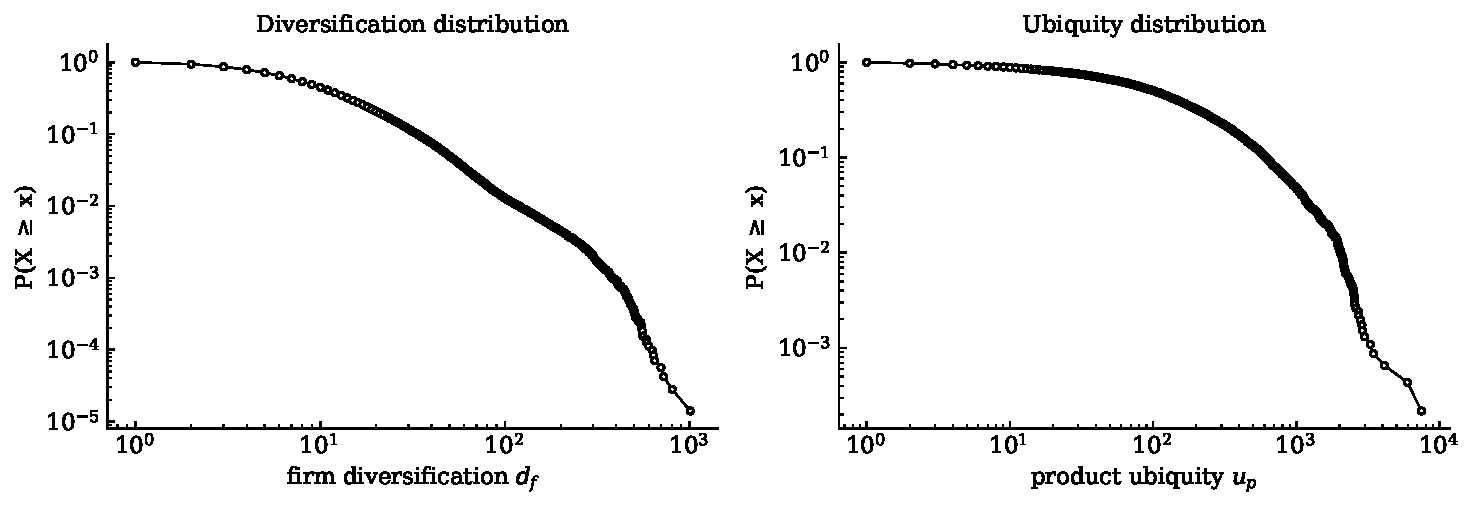
\includegraphics[width=0.92\textwidth]{ds_fig1_distributions.pdf}
\caption{Complementary CDFs of firm diversification $d_f$ (left) and product ubiquity $u_p$ (right), on
log--log axes.}
\label{fig:dist}
\end{figure}

%=================================================================
\subsection{Community detection}

Standard modularity (Newman, 2006) and its bipartite (Barber, 2007) counterpart for a firm$\times$product
incidence $B$, with firm degrees $k$, product degrees $d$ and $m=\sum_{fp}B_{fp}$, are
\begin{equation}
Q=\frac{1}{2m}\sum_{ij}\Big(A_{ij}-\tfrac{k_ik_j}{2m}\Big)\delta(c_i,c_j),
\qquad
\QB=\frac{1}{m}\sum_{fp}\Big(B_{fp}-\tfrac{k_f d_p}{m}\Big)\delta(g_f,g_p).
\end{equation}
Louvain and Leiden optimise the standard $Q$ on the bipartite graph; BRIM optimises $\QB$, the correct
bipartite null, and is De Stefano's choice, which we carry forward as canonical. Table~\ref{tab:algos} compares
the three.

\begin{table}[H]\centering\small
\caption{Community detection on the same incidence (late-8, HS6). All at resolution $\gamma=1$.}
\label{tab:algos}
\begin{tabular}{@{}lcc@{}}
\toprule
Algorithm & \#blocks & $\QB$ \\
\midrule
Louvain & 13 & 0.521 \\
Leiden  &  9 & 0.538 \\
\textbf{BRIM (canonical)} & \textbf{5} & \textbf{0.505} \\
\midrule
\multicolumn{3}{l}{\emph{De Stefano (Italy): 7 blocks, $\QB=0.501$}}\\
\bottomrule
\end{tabular}
\qquad
\begin{tabular}{@{}lcc@{}}
\toprule
Agreement (firm side) & ARI & NMI \\
\midrule
Louvain vs Leiden & 0.558 & 0.669 \\
Louvain vs BRIM   & 0.425 & 0.584 \\
Leiden vs BRIM    & 0.455 & 0.615 \\
\bottomrule
\end{tabular}
\end{table}

The headline is that our BRIM modularity, $\QB=0.505$, is essentially identical to their $0.501$: the
\emph{strength} of the modular structure replicates almost exactly across two very different economies. The
\emph{number} of blocks, by contrast, is not an invariant --- it depends on the algorithm (Louvain and Leiden
over-segment bipartite graphs) and on the resolution $\gamma$ (on this same network the count runs
$5\to10\to24\to70$ as $\gamma=1\to2\to4\to8$). The comparison with their seven is therefore meaningful only at
the same $\gamma=1$ and the same (BRIM) algorithm, a point worth remembering before reading anything into ``5
vs 7''.

\paragraph{What $\gamma$ is.} The resolution $\gamma$ weights the null term in the modularity. Each pair of
nodes placed in the same block is ``charged'' $\gamma$ times its expected random-baseline connection
$k_f d_p/m$, against a reward of $+1$ per observed link; a block survives only when its internal reward beats
that charge. So $\gamma=1$ is standard modularity --- the charge equals the configuration-model expectation,
De Stefano's choice --- while $\gamma>1$ raises the charge and yields more, smaller blocks, and $\gamma<1$
yields fewer, larger ones. In the CPM-bipartite implementation we use, $\gamma$ is equivalently a
\emph{density threshold}: a community is kept only if its internal link density exceeds $\gamma$. The Leiden
routine is only the optimiser; $\gamma$ is a property of the objective, not of the algorithm. The Appendix
details the three algorithms and their null models. We keep $\gamma=1$ throughout and report $\gamma=2$ as a
robustness check (\S\ref{sec:gamma}).

%=================================================================
\subsection{Block anatomy and the De Stefano comparison}

\subsubsection{What our blocks contain}
Table~\ref{tab:blocks} reports the five BRIM blocks with their dominant HS chapters and representative products.

\begin{table}[H]\centering\small
\caption{The five BRIM blocks (late-8, HS6; $71{,}017$ firms).}
\label{tab:blocks}
\begin{tabular}{@{}clp{6.8cm}@{}}
\toprule
Block & Firms & Dominant content \\
\midrule
0 & 36{,}321 (51\%) & Machinery \& electrical 36\%, base metals 24\%, instruments 7\% --- the large \emph{generalist} block (absorbs electrical machinery) \\
2 & 16{,}095 (23\%) & Paper 16\%, misc.\ manufacturing 12\%, packaging/cases --- light manufacturing \\
1 & 10{,}870 (15\%) & \textbf{Textiles 95\%} --- apparel, cotton, man-made fibres (pure) \\
3 &  7{,}691 (11\%) & \textbf{Chemicals 48\% + agri-food $\sim$41\%} (vegetables 18\%, foodstuffs 12\%, animals 11\%) \\
4 &     40 (0\%)    & Precious 100\% --- diamonds (pure satellite) \\
\bottomrule
\end{tabular}
\end{table}

\begin{figure}[H]\centering
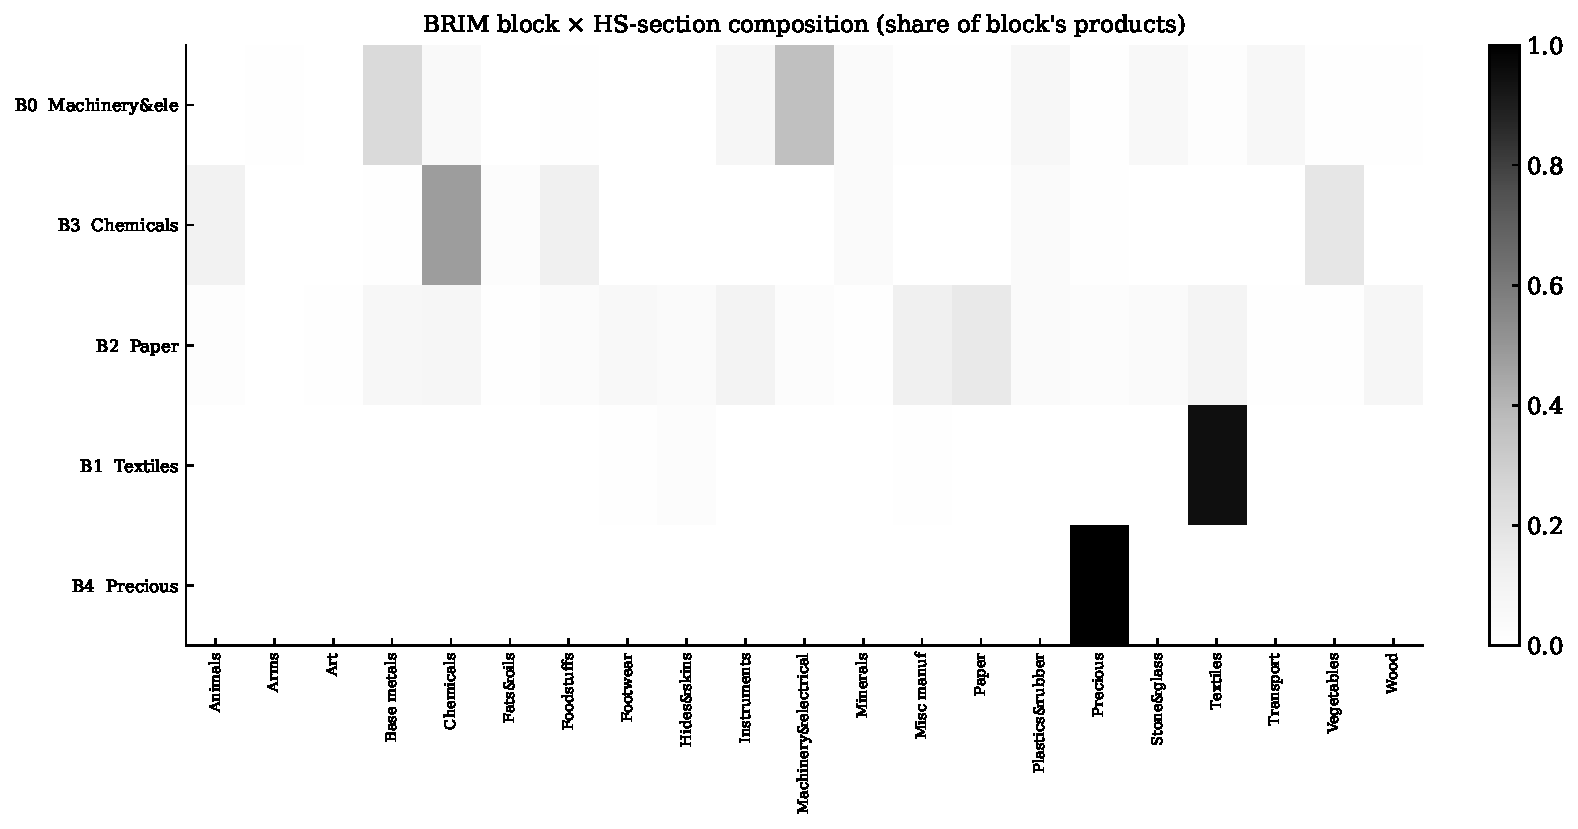
\includegraphics[width=0.95\textwidth]{ds_fig2_block_sections.pdf}
\caption{BRIM block $\times$ HS-section composition (share of each block's products in each section).
Textiles (block 1) is near-pure; the generalist block 0 spreads across machinery, metals and instruments.}
\label{fig:blocksec}
\end{figure}

\subsubsection{Comparison with De Stefano's seven blocks}
The mapping in Table~\ref{tab:compare} shows the differences are economically sensible rather than failures of
replication.

\begin{table}[H]\centering\footnotesize
\caption{Block-by-block comparison (validation).}
\label{tab:compare}
\begin{tabular}{@{}p{5.0cm}p{5.0cm}c@{}}
\toprule
De Stefano (Italy, 7) & Ours (China, 5) & Match \\
\midrule
Machinery \& metal (largest, $\sim$30\%) & Block 0 ($\sim$51\%): machinery, metals \emph{+ electrical} & \checkmark\ larger, absorbs electrical \\
Electrical machinery (TVs, hard disks)   & folded into Block 0                       & $\times$ does not separate \\
Chemicals \& minerals                    & Block 3 (chemicals 48\% + agri-food)      & \checkmark\ chemicals; food bundled in \\
Paper \& plastic                         & Block 2 (paper, packaging, light mfg)     & \checkmark\ partial \\
Textile products                         & Block 1 (cotton, apparel)                 & \checkmark\ strong, pure \\
Food \& animals                          & bundled into Block 3                      & $\sim$ no \emph{standalone} food block \\
Wood/glass/jewelry (least interpretable) & Block 4 (diamonds, 40 firms)              & $\sim$ partial \\
\bottomrule
\end{tabular}
\end{table}

Three economically robust pillars --- textiles, chemicals, machinery/metals --- emerge in both countries with
coherent content and near-identical $\QB$, so the block structure is not a country artefact. Where China
differs, it differs for a reason: machinery, metals and electronics collapse into one large generalist block
($\sim$51\% of firms, the ``factory of the world'' assembly base), and agri-food does not nucleate its own
cluster but bundles with chemicals. This yields five blocks rather than seven --- a \emph{merging} difference,
at the same modularity.

\subsubsection{The De Stefano robustness check}
We cannot run their growth regression (we have no firm outcomes), so we test the same claim at the partition
level: the BRIM product-partition against the HS-section partition gives $\mathrm{ARI}=0.289$ and
$\mathrm{NMI}=0.426$, with blocks spanning on average thirteen HS sections (min 1, max 21). The data-driven
partition is therefore not a relabelling of HS sectors --- exactly their Table~2 point, reproduced.

%=================================================================
\subsection{In-block and out-of-block diversification}

With $\delta_{fp}=\mathbb{1}\{\text{block}(f)=\text{block}(p)\}$, the diversification split is
\begin{equation}
\din_f=\sum_p M_{fp}\,\delta_{fp},\quad
\dout_f=\sum_p M_{fp}(1-\delta_{fp}),\quad
d_f=\din_f+\dout_f,\quad
\mathrm{Share}^{\mathrm{in}}_f=\frac{\din_f}{d_f}.
\end{equation}
In words, $\din$ counts a firm's competitive (RCA$>1$) products that lie \emph{inside} its own capability
block, $\dout$ those \emph{outside} it, and the share is the proportion staying in-block.
Table~\ref{tab:div} reports the distribution.

\begin{table}[H]\centering\small
\caption{Diversification indicators, late-8 / HS6 ($N=71{,}017$ active firms).}
\label{tab:div}
\begin{tabular}{@{}lrrrrrrr@{}}
\toprule
 & mean & sd & p10 & p25 & median & p75 & p90 \\
\midrule
$\din$              & 13.01 & 20.83 & 2 & 4 & 7 & 14 & 29 \\
$\dout$             &  2.53 & 11.38 & 0 & 0 & 0 &  2 &  5 \\
$d$                 & 15.54 & 28.53 & 2 & 4 & 8 & 17 & 33 \\
$\mathrm{Share}^{\mathrm{in}}$ & 0.888 & 0.162 & 0.63 & 0.80 & 1.00 & 1.00 & 1.00 \\
\bottomrule
\end{tabular}

\smallskip
\footnotesize Pure in-block ($\mathrm{Share}^{\mathrm{in}}=1$): 54.5\%; pure out-of-block: 0\%; mixed: 45.5\%.
\end{table}

The picture is one of deep specialisation. In-block diversification dominates; $\dout$ is zero for $54.5\%$ of
firms (equivalently, $\mathrm{Share}^{\mathrm{in}}=1$ for that majority), and where it is positive it is
small. Reading the right panel of Fig.~\ref{fig:div}, firms grow along the $\din$ axis, within their block,
which is the exploitation--exploration language of March (1991): these established Chinese exporters are
exploitation-heavy. That zero-inflation and that ceiling at $\mathrm{Share}^{\mathrm{in}}=1$ are not just
descriptive curiosities --- they are the central fact a dynamic model of these outcomes will have to confront,
and we come back to them in the final section.

\begin{figure}[H]\centering
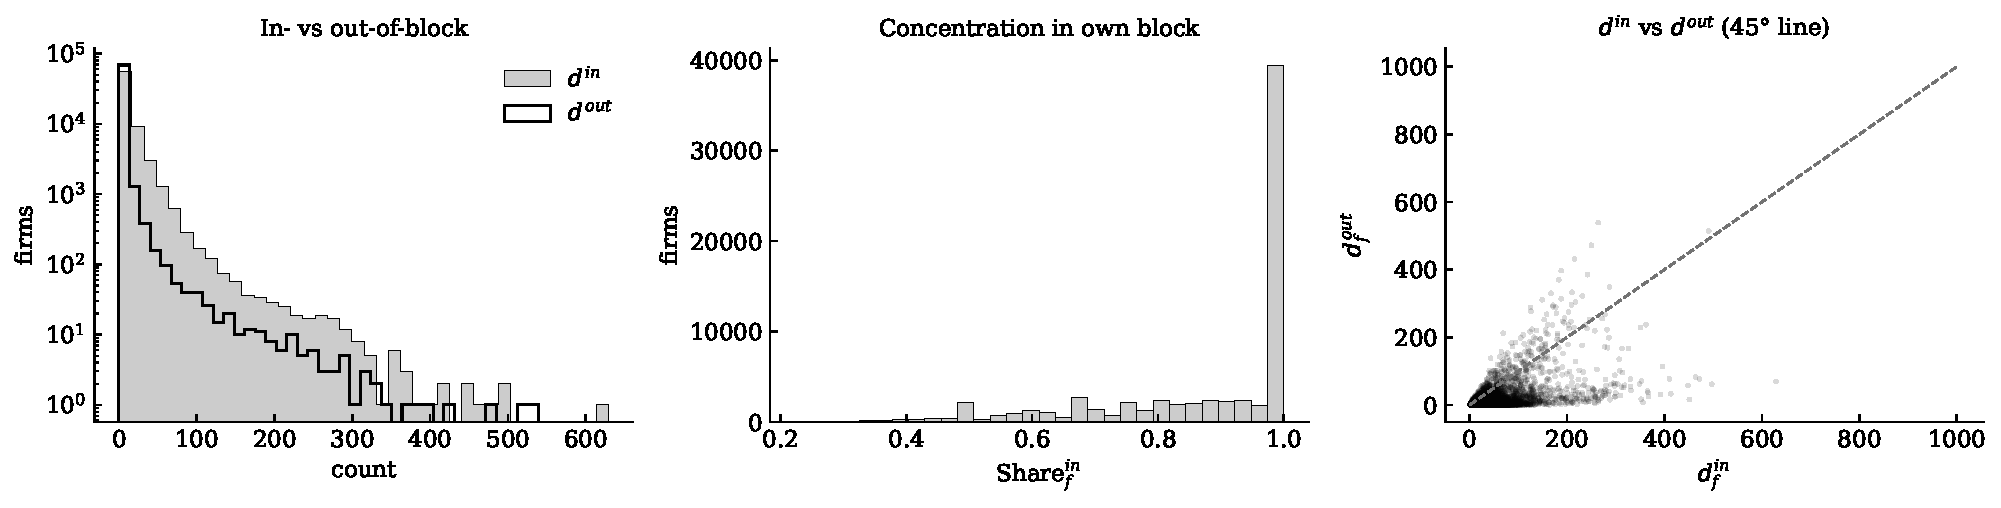
\includegraphics[width=0.99\textwidth]{ds_fig3_diversification.pdf}
\caption{\textbf{Left:} in- vs out-of-block diversification (log $y$). $\din$ dominates; $\dout$ is
zero for $54.5\%$ of firms (the median firm has $\dout=0$). \textbf{Centre:} concentration
$\mathrm{Share}^{\mathrm{in}}$ --- a mass of $54.5\%$ at $1$ (pure specialists, equivalently $\dout=0$).
\textbf{Right:} $\din$ vs $\dout$ with the $45^\circ$ line; the cloud lies below it, firms grow along the
$\din$ axis.}
\label{fig:div}
\end{figure}

%=================================================================
\subsection{Coherence and Fitness}

\paragraph{Coherence (Sapling Similarity).}
$C_f=\sum_{p,p'}E_{fp}E_{fp'}B_{pp'}\big/\big(\sum_p E_{fp}\big)^2$ with the Sapling kernel $B$ (Albora et al.,
2023), computed for $68{,}434$ firms (top-1500 products), with mean $0.626$ and range $[0.02,1.00]$. As one
would expect, more diversified firms have somewhat \emph{lower} coherence (Fig.~\ref{fig:coh}): broader baskets
are less internally related.

\begin{figure}[H]\centering
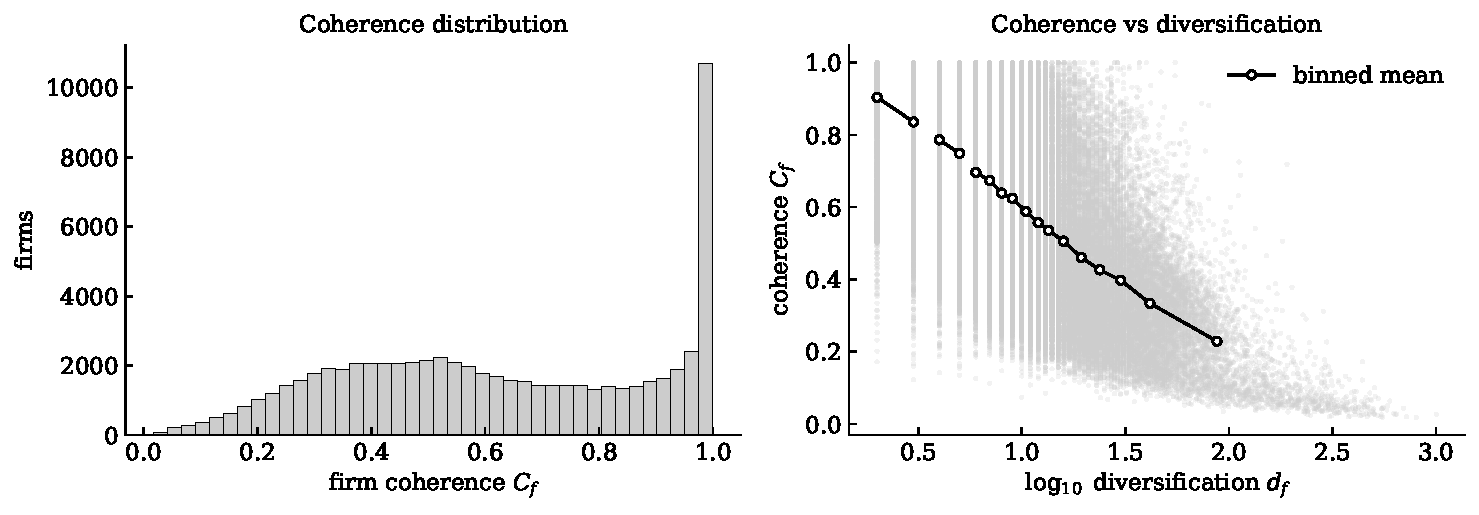
\includegraphics[width=0.92\textwidth]{ds_fig4_coherence.pdf}
\caption{Distribution of firm coherence $C_f$ (left) and coherence vs.\ diversification with binned mean
(right).}
\label{fig:coh}
\end{figure}

For De Stefano coherence is a descriptive indicator; for us it will do identifying work in the dynamic
extension, and it is worth saying why now. \textbf{Export intermediaries} --- trading companies and
wholesalers --- carry baskets of \emph{unrelated} products, shipping whatever crosses their desk rather than a
capability-driven portfolio. They therefore display artificially high $\dout$ and very \emph{low} coherence.
Left uncontrolled, they would masquerade as ``explorers'' and contaminate the out-of-block signal precisely
where the dynamic story lives. Coherence $C_f$ flags them: conditioning on it, or trimming the low-coherence
tail, separates genuine capability reconfiguration from intermediary churn. That is why we compute it now, even
though it is not part of the headline replication.

\paragraph{Fitness--Complexity (Tacchella et al., 2012).}
The non-linear map, iterated to a fixed point, is
\begin{equation}
F_f^{(n)}=\sum_p M_{fp}\,Q_p^{(n-1)},\qquad
Q_p^{(n)}=\frac{1}{\sum_f M_{fp}\big/F_f^{(n-1)}}.
\end{equation}
We reproduce the indicator (Fig.~\ref{fig:fit}); fitness rises with diversification but not one-for-one. We
cannot test their Appendix-C finding that complexity does not predict growth, since that needs firm outcomes.

\begin{figure}[H]\centering
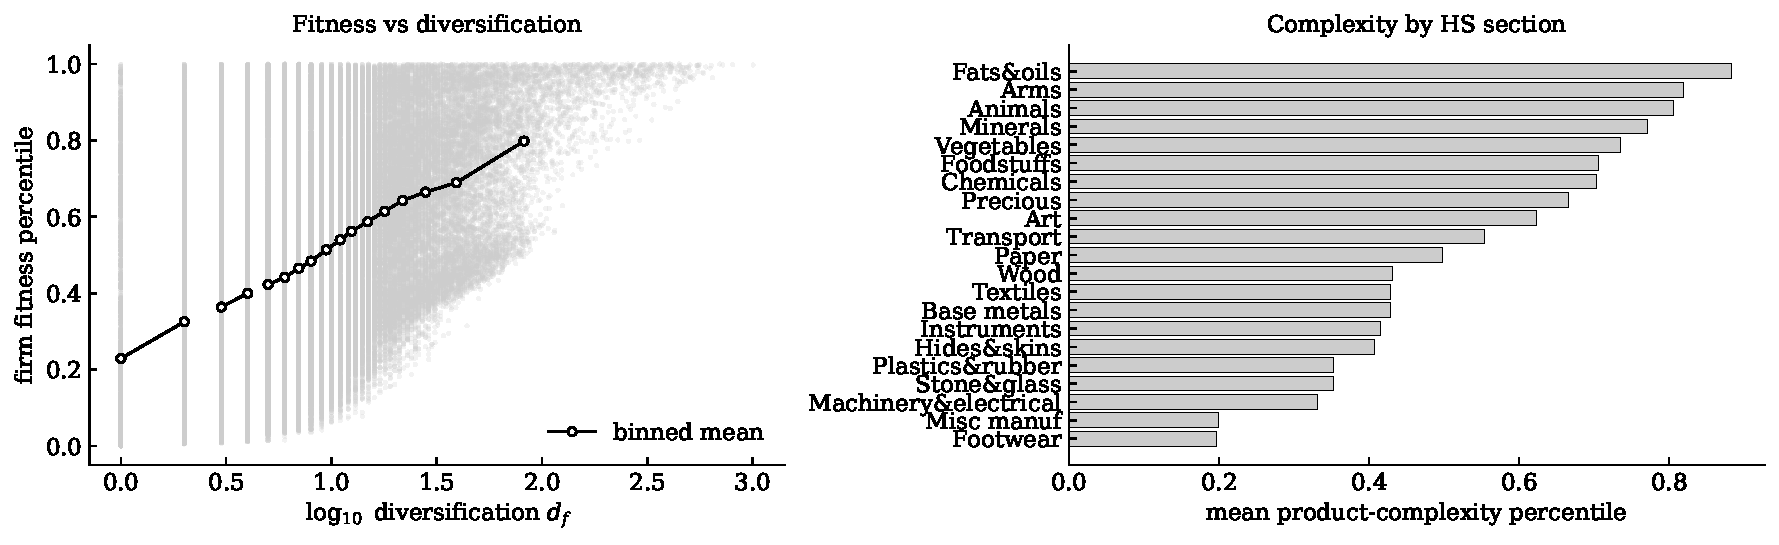
\includegraphics[width=0.92\textwidth]{ds_fig5_fitness.pdf}
\caption{Firm fitness vs.\ diversification (left, binned mean) and mean product complexity by HS section
(right).}
\label{fig:fit}
\end{figure}

\paragraph{What we cannot replicate.} Two parts of De Stefano's analysis require data outside a single
country's firm exports, and we flag them honestly rather than approximate them. EXPY and PRODY
(Hausmann--Hwang--Rodrik, 2007) are built from the \emph{world} country--product matrix and GDP per capita; a
single country's firm exports give no cross-country variation to estimate PRODY. The growth and
profit-per-employee regressions need ORBIS firm financials, which we do not have. Everything else --- RCA,
BRIM, $\din/\dout$, coherence, fitness --- is computed exactly as they describe.

%=================================================================
\section{Extension I --- Who explores out of block? Destinations and the multinational reading}
\label{sec:dest}

De Stefano stop at the firm--product layer. Our microdata also carry the export \emph{destination}, which lets
us give $\dout$ an economic identity, and ask the question that matters for what comes next: are the out-of-block
explorers the wide-reaching, ``multinational-like'' exporters? For each firm we measure \emph{destination reach}
$n^{\mathrm{dest}}_f$ (the number of distinct destination countries served over 2008--2015) and \emph{flow}
(total export value), and cut the $71{,}017$ firms into $5\times5$ quintiles of flow $\times$ reach.

The headline is a contrast of two correlations. Out-of-block diversification correlates with destination reach
at $0.18$, but with export value at only $0.03$ (Spearman). Reaching more markets tracks out-of-block
exploration; sheer revenue does not. Table~\ref{tab:destgrid} makes the pattern transparent on the size-free out-of-block share:
reading \emph{across} a row, toward more destinations, the share rises monotonically at every flow level;
reading \emph{down} a column, toward more volume, it falls. Importantly, along the destination axis the
absolute count $\dout$ and the share move together --- both rise with reach in every flow row --- so
destinations are unambiguous. The count-versus-share tension appears only on the flow axis, where the count
rises but the share falls; we explain that next.

\begin{table}[H]\centering\small
\caption{Out-of-block share \% by export-flow quintile (rows, F1 low $\to$ F5 high) $\times$
destination-reach quintile (columns), late-8 / HS6. Median destinations per column:
D1$\approx$3, D2$\approx$9, D3$\approx$17, D4$\approx$30, D5$\approx$54.}
\label{tab:destgrid}
\begin{tabular}{@{}lrrrrr@{}}
\toprule
Export flow & D1 & D2 & D3 & D4 & D5 \\
\midrule
F1 (low)  & 10.0 & 11.5 & 13.1 & 14.0 & 14.8 \\
F2        &  8.7 & 10.5 & 12.1 & 13.9 & 16.3 \\
F3        &  7.7 &  8.8 & 10.5 & 13.0 & 15.2 \\
F4        &  7.6 &  8.1 &  9.6 & 11.5 & 14.6 \\
F5 (high) &  7.4 &  7.3 &  8.5 &  9.6 & 13.7 \\
\bottomrule
\end{tabular}

\smallskip
\footnotesize Across a row (more destinations) the share rises; down a column (more volume) it falls.
Breadth tilts the portfolio outward; volume tilts it inward.
\end{table}

The raw count tells a complementary story (Fig.~\ref{fig:dest}, left, log scale): the flow lines overlap across
the first four destination quintiles and fan out only in the last, where the top-flow line jumps from
$\dout\approx1.05$ in the low-flow/few-destination corner to $7.3$ in the high-flow/many-destination corner, a
factor of seven. But the difference-in-differences across the corners is $+2.9$ products on the count and only
$+1.5$ pp on the size-free share, so the apparent ``synergy'' of being both large and broad is largely the
big-and-broad firms simply being large. On the proportion the flow lines stay roughly parallel, with no strong
size-free complementarity.

\begin{figure}[H]\centering
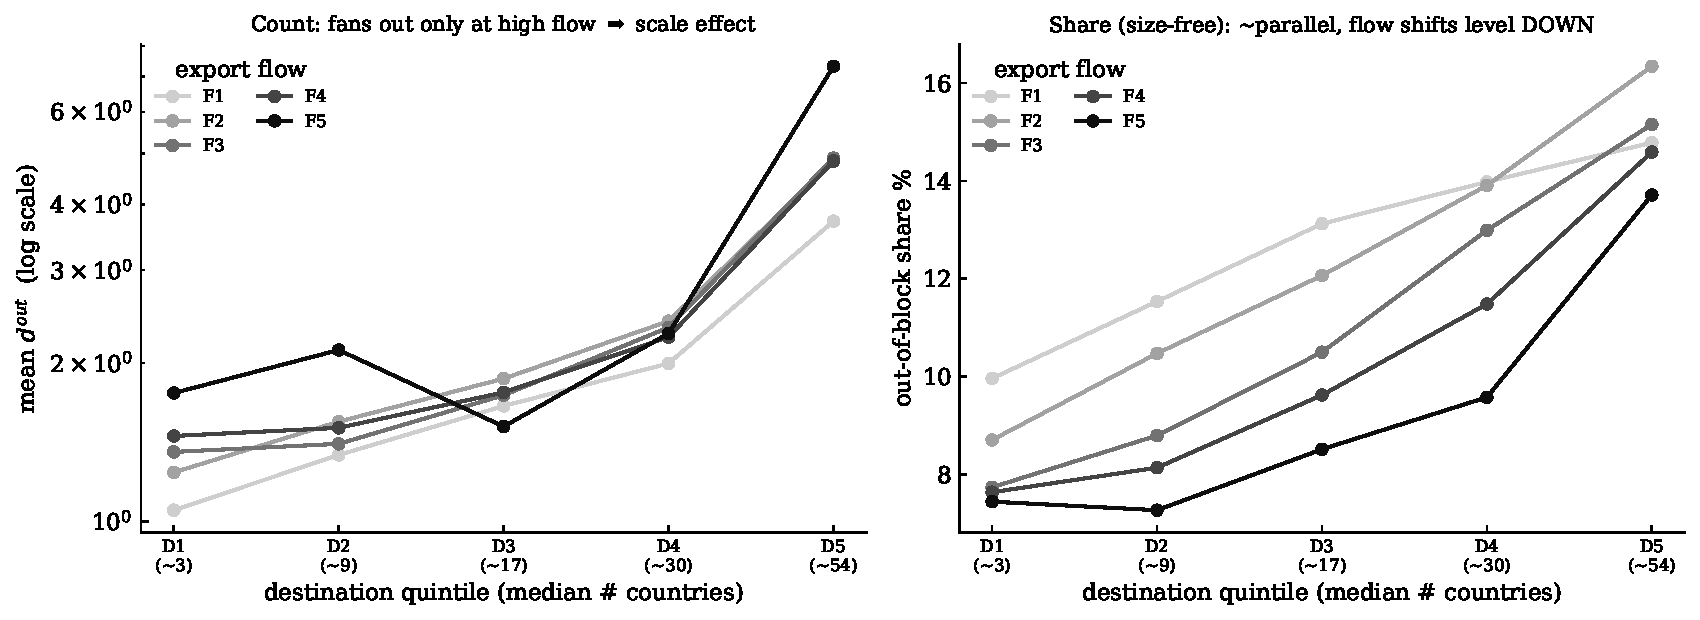
\includegraphics[width=0.99\textwidth]{ds_fig6_dest_interaction.pdf}
\caption{Out-of-block exploration by export flow $\times$ destination reach (five flow quintiles,
light $=$ low to dark $=$ high flow). \textbf{Left:} mean $\dout$ count (log scale) --- every line rises with
destinations; the lines additionally fan out at the highest destination quintile (a scale effect).
\textbf{Right:} size-free out-of-block share --- every flow line again rises with destinations, and the
high-flow lines sit \emph{below}. Both panels rise along the destination axis; they part only on the flow axis.}
\label{fig:dest}
\end{figure}

That volume should \emph{lower} the share looks paradoxical --- shouldn't bigger firms do more of everything?
They do, in absolute terms; the subtlety is on the proportion. Holding destination reach fixed, going from the
lowest to the highest flow quintile raises both margins ($\din$ $\times1.86$, $\dout$ $\times1.53$), but $\din$
grows more in proportion, so the out-of-block share falls from $12.7\%$ to $9.3\%$ (Fig.~\ref{fig:mech}). The
reason is that RCA is scale-invariant: a high-value firm is not just ``the same firm, bigger'' but one with a
more core-concentrated product mix. Scaling in export value comes from deepening in the core --- specialisation
--- not from scattering into unrelated products. Geographic breadth and export volume are therefore different,
opposing margins: the extensive margin of markets pushes the portfolio out of block, the intensive margin of
value pulls it in. This mechanism is, however, the \emph{least robust} of our findings: it is clean and
monotone at $\gamma=1$ but partially reverses at the highest flow quintile under the finer $\gamma=2$ partition
(\S\ref{sec:gamma}), so we read it as a $\gamma=1$ pattern rather than a law. The destination result above does
not have this fragility --- it is monotone at both resolutions.

\begin{figure}[H]\centering
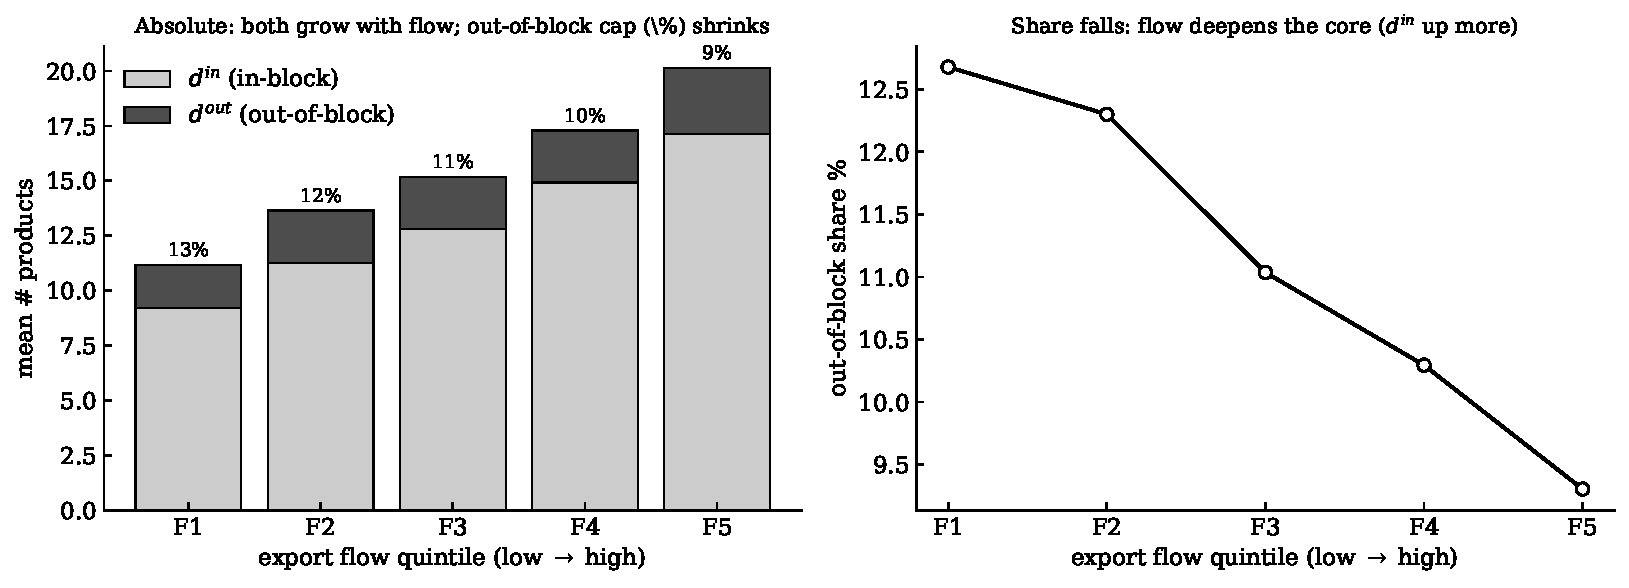
\includegraphics[width=0.97\textwidth]{ds_fig7_flow_mechanism.pdf}
\caption{Flow mechanism, destination reach held fixed (equal-weight average over destination quintiles).
\textbf{Left:} stacked $\din+\dout$ by flow quintile --- the basket grows but the out-of-block cap thins from
$13\%$ to $9\%$. \textbf{Right:} the out-of-block share falls with flow: scaling in value deepens the core.}
\label{fig:mech}
\end{figure}

Economically this is again the exploration--exploitation logic of March (1991). Exploring outside one's
capability block is costly, and it is the firms exposed to many heterogeneous markets --- and with the
organisational slack to act on that exposure --- that do it, not the firms that simply pump volume through their
core. So $\dout$ is the signature of the wide-reach exporter, not the big-revenue one. The ``multinational-like''
type, if we want to talk about one, should be defined on geographic breadth; defining it on volume is not what
the data support.

%=================================================================
\section{Extension II --- Where $\dout$ lives: across the capability blocks}
\label{sec:blocks}

Having seen \emph{which firms} explore, we ask \emph{which blocks} they sit in. Table~\ref{tab:blockdiv}
distributes $\din$, $\dout$ and the out-of-block share across the five BRIM blocks, with each block's median
reach, median export and product count. One structural caveat is needed to read it: the out-of-block share
depends mechanically on block size, because a firm in a large block has a big in-block menu and so few of its
products fall outside, whereas a firm in a small, pure block has few in-block options and a larger share out by
construction.

\begin{table}[H]\centering\footnotesize
\caption{In-/out-of-block diversification by BRIM block (sorted by out-of-block share). Export in raw USD.}
\label{tab:blockdiv}
\setlength{\tabcolsep}{5pt}
\begin{tabular}{@{}lrrrrrrr@{}}
\toprule
Block & firms & $\din$ & $\dout$ & share$^{\mathrm{out}}$ & med.\ dest & med.\ exp.\ & \#prod. \\
\midrule
B2 Paper / light-mfg     & 16{,}095 &  8.56 & 4.46 & 21.5\% & 22 & \$12.0M & 715 \\
B3 Chemicals + agri-food &  7{,}691 &  9.01 & 1.50 &  9.0\% & 14 & \$19.9M & 1{,}173 \\
B1 Textiles              & 10{,}870 & 24.55 & 3.10 &  8.6\% & 15 & \$21.0M & 698 \\
B0 Machinery \& electr.  & 36{,}321 & 12.39 & 1.73 &  7.9\% & 17 & \$14.9M & 1{,}995 \\
B4 Precious (diamonds)   &      40  &  1.55 & 0.02 &  0.6\% &  3 & \$57.8M & 5 \\
\bottomrule
\end{tabular}
\end{table}

Even with that caveat, the blocks sort into recognisable firm types. \textbf{Paper / light manufacturing
(B2)} is the explorer block by a wide margin: an out-of-block share of $21.5\%$ and $\dout=4.46$, roughly three
times every other block, on firms that also reach the most markets (median 22 destinations). \textbf{Textiles
(B1)} is the opposite --- a $\din$ of $24.6$, the highest by far, yet an out-of-block share of only $8.6\%$:
textile firms diversify enormously, but \emph{within} textiles (yarns, fabrics, the many apparel lines), not
outside. \textbf{Precious / diamonds (B4)} is the limiting case of the volume story from \S\ref{sec:dest}: the
highest median export of all (\$57.8M) but only three destinations and essentially no out-of-block activity ---
a few large, ultra-specialised intensive-margin traders. \textbf{Machinery (B0)} and \textbf{chemicals (B3)}
are the big generalist blocks, with structurally lower out-of-block shares because their in-block menus (1{,}995
and 1{,}173 products) are so large.

It is worth pausing on the contrast between Textiles and Machinery, because at first glance it looks
contradictory: Textiles has a \emph{higher} $\din$ ($24.6$ vs $12.4$) despite a \emph{smaller} block ($698$ vs
$1{,}995$ products). The resolution is that block size is an aggregate property --- how many distinct products
exist in the block across all firms --- while $\din$ is per firm. A textile firm covers about $3.5\%$ of its
block's products ($24.6/698$); a machinery firm only $0.6\%$ ($12.4/1{,}995$). Textiles is a narrow, deep block
of closely related lines that each firm makes many of; machinery is a wide, shallow galaxy of heterogeneous
niches, large in total but sparse per firm.

\begin{figure}[H]\centering
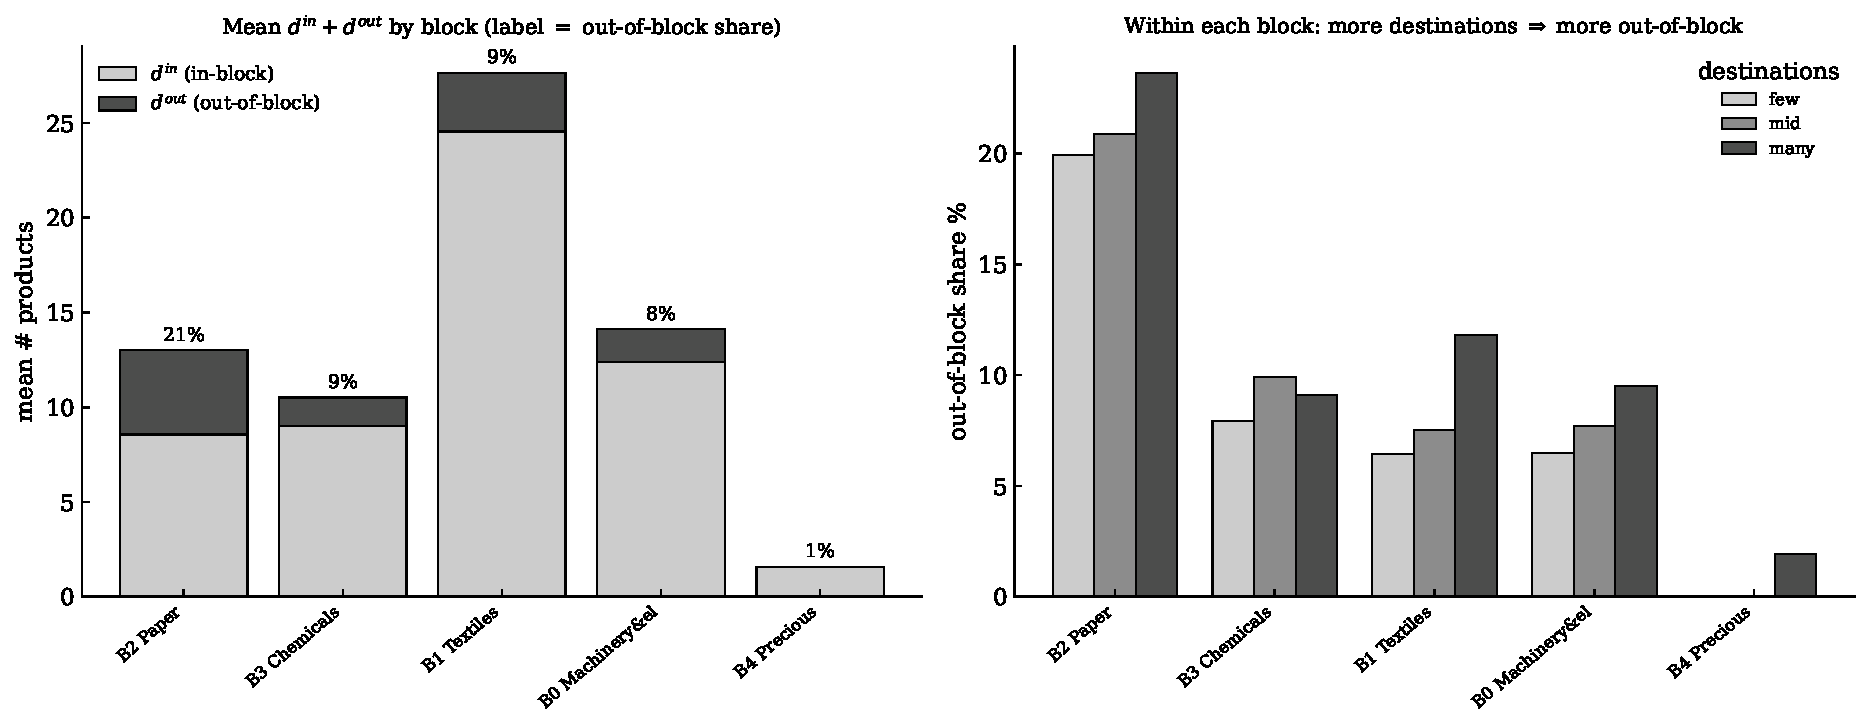
\includegraphics[width=0.99\textwidth]{ds_fig8_blocks.pdf}
\caption{\textbf{Left:} mean $\din+\dout$ by block (label $=$ out-of-block share); the out-of-block cap is by
far thickest for Paper. \textbf{Right:} out-of-block share by within-block destination tercile (few/mid/many).
The ``more destinations $\Rightarrow$ more out-of-block'' pattern holds inside every block, so it is not an
artefact of composition across blocks.}
\label{fig:blocks}
\end{figure}

The right panel of Fig.~\ref{fig:blocks} adds a reassuring robustness check: the destination gradient of
\S\ref{sec:dest} reappears \emph{within} each block --- more destinations means a higher out-of-block share in
Paper, Textiles, Machinery and (more weakly) Chemicals alike. The link between geographic breadth and
out-of-block exploration is therefore not a between-block composition effect; it operates inside each capability
community.

\subsection{Resolution robustness: $\gamma=1$ vs $\gamma=2$}
\label{sec:gamma}

The block \emph{count} depends on the resolution parameter $\gamma$, which weights the bipartite null in the
modularity. De Stefano use standard modularity, $\gamma=1$, which we keep as the baseline of the whole note; to
check that the substantive findings do not hinge on it, we re-ran the \emph{entire} pipeline at $\gamma=2$ --- a
finer resolution that penalises the null more, and so yields more, smaller blocks. Table~\ref{tab:gamma} puts
the two side by side.

\begin{table}[H]\centering\small
\caption{The same pipeline at two resolutions. Levels rescale; conclusions do not.}
\label{tab:gamma}
\begin{tabular}{@{}lcc@{}}
\toprule
Quantity & $\gamma=1$ (baseline) & $\gamma=2$ \\
\midrule
BRIM blocks                         & 5      & 10     \\
Bipartite modularity $\QB$          & 0.505  & 0.544  \\
ARI vs HS sections                  & 0.289  & 0.318  \\
NMI vs HS sections                  & 0.426  & 0.476  \\
HS sections spanned per block (avg) & 13     & 9.4    \\
Block purity (mean dominant chapter)& 59\%   & 66\%   \\
Pure in-block (Share$^{\mathrm{in}}=1$) & 54.5\% & 43.2\% \\
$\mathrm{corr}(\dout,\text{reach})$ & 0.18   & 0.16   \\
$\mathrm{corr}(\dout,\text{value})$ & 0.03   & 0.06   \\
\bottomrule
\end{tabular}
\end{table}

Doubling the resolution splits the five blocks into ten and raises modularity ($\QB$: $0.505\to0.544$), as
expected. The split is partly meaningful and partly mechanical. \textbf{Meaningful:} agri-food, bundled into the
chemicals block at $\gamma=1$, separates into its own block at $\gamma=2$ (vegetables/animals/foodstuffs), and
dedicated footwear and transport blocks emerge; HS-sections-per-block falls from 13 to 9.4 and per-block purity
rises. \textbf{Mechanical:} the coherent textile block splits into two near-identical pure-textile sub-blocks
(over-segmentation), and the machinery--metals core stays mixed at any resolution --- firm-weighted purity
barely moves ($42\%\to45\%$), because the bulk of firms sit in that entangled generalist block.
Table~\ref{tab:gammamap} traces how each $\gamma=1$ block maps to its $\gamma=2$ descendants, and
Fig.~\ref{fig:g2sec} shows the ten finer blocks against HS sections (to be read against Fig.~\ref{fig:blocksec}).

\begin{table}[H]\centering\footnotesize
\caption{How the five $\gamma=1$ blocks split at $\gamma=2$.}
\label{tab:gammamap}
\begin{tabular}{@{}p{4.6cm}p{6.3cm}p{3.2cm}@{}}
\toprule
$\gamma=1$ block & $\to$ $\gamma=2$ descendants & nature \\
\midrule
B0 machinery generalist (51\%) & machinery+metals (30\%), machinery+instruments (15\%), transport & core stays mixed; instruments/transport peel off \\
B3 chemicals + agri-food (11\%) & chemicals 65\%, \emph{agri-food} (own block) & genuine separation \\
B1 textiles 95\% (15\%) & two pure-textile blocks (90\%, 97\%) & over-split (artefact) \\
B2 paper/light-mfg catch-all (23\%) & catch-all (27\%), footwear & footwear peels off \\
B4 precious (0\%) & precious (unchanged) & unchanged \\
\bottomrule
\end{tabular}
\end{table}

\begin{figure}[H]\centering
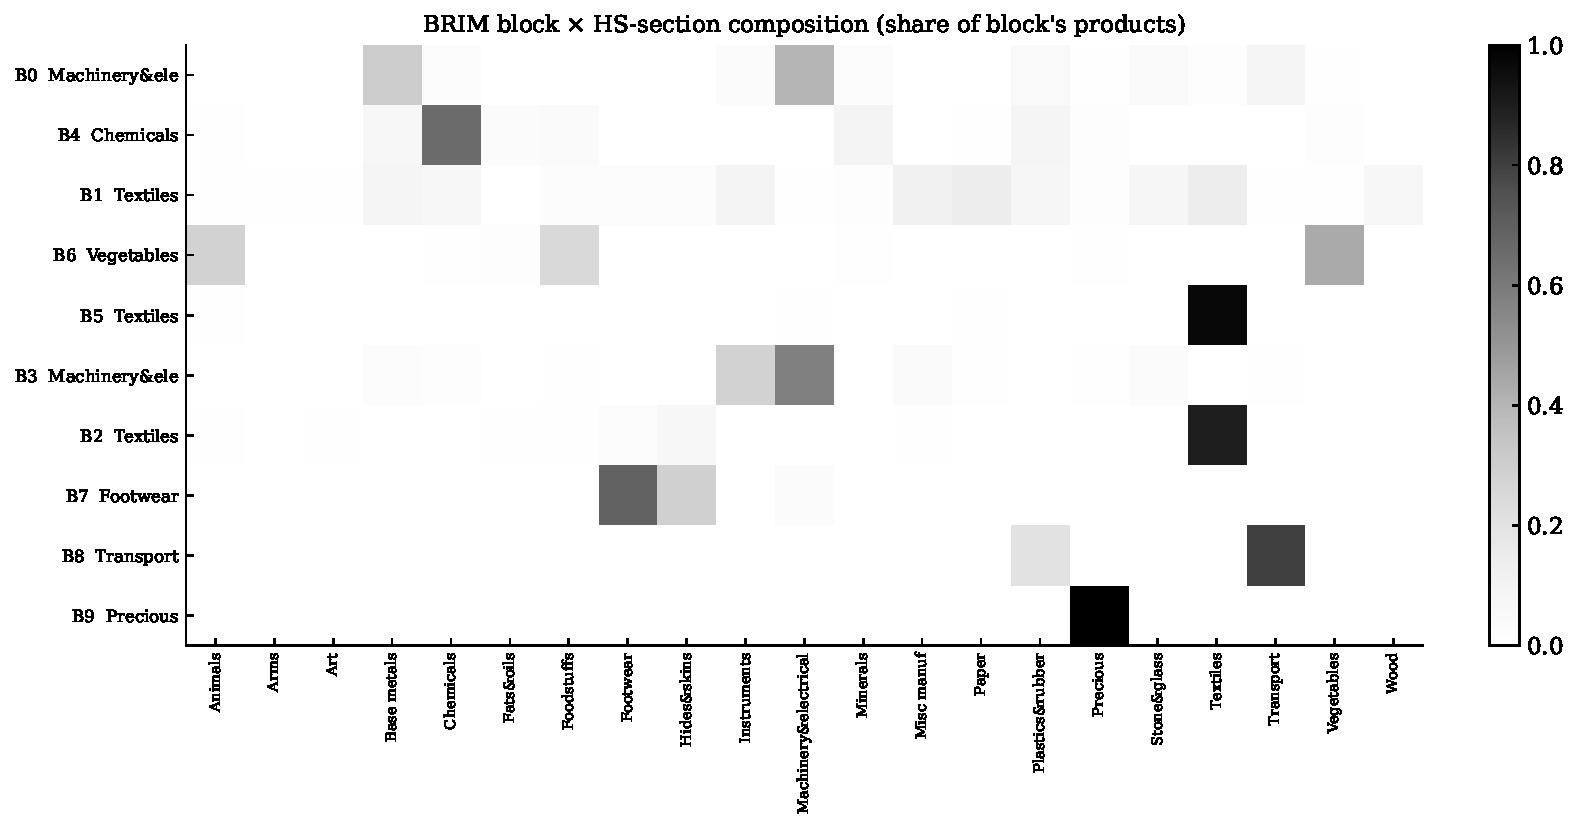
\includegraphics[width=0.92\textwidth]{ds_g2_block_sections.pdf}
\caption{$\gamma=2$: BRIM block $\times$ HS-section composition (ten blocks). Pure blocks show as isolated dark
cells --- textiles (two), chemicals, footwear, transport, precious --- while block 0 (machinery+metals) and the
catch-all block 1 stay spread. Compare with the five-block $\gamma=1$ map, Fig.~\ref{fig:blocksec}.}
\label{fig:g2sec}
\end{figure}

\begin{figure}[H]\centering
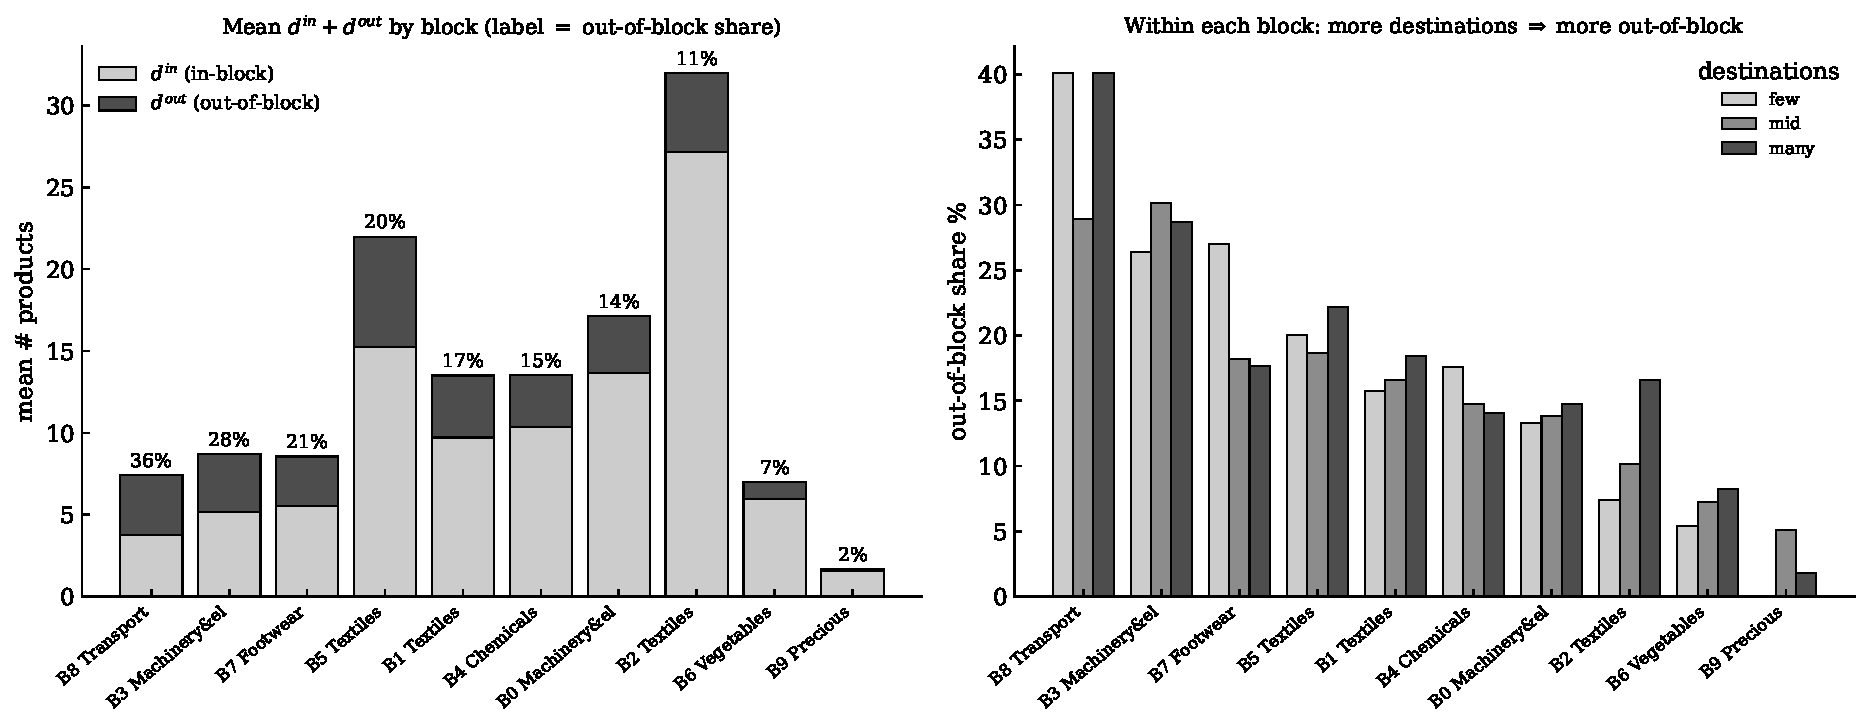
\includegraphics[width=0.99\textwidth]{ds_g2_blocks.pdf}
\caption{$\gamma=2$: in-/out-of-block diversification by block (left) and the within-block destination gradient
(right). As at $\gamma=1$ (Fig.~\ref{fig:blocks}), out-of-block exploration still rises with destination reach
inside the blocks; the absolute shares are uniformly higher because the finer blocks have smaller in-block
menus.}
\label{fig:g2blocks}
\end{figure}

\paragraph{The conclusions survive; only the levels rescale.} Finer blocks mean a smaller in-block menu, so the
out-of-block share rises across the board (pure in-block $54.5\%\to43.2\%$) and is \emph{not} comparable across
$\gamma$ --- read $\dout$ levels within a resolution, never across. But every substantive conclusion holds at
$\gamma=2$: the modular structure is real and in fact stronger ($\QB$ higher); the blocks are still not a
relabelling of HS sectors (ARI/NMI rise only marginally, to $0.32/0.48$, and stay far below $1$ --- the finer
blocks are slightly more sector-like, as one would expect, but nowhere near a relabelling); and out-of-block
exploration still tracks destination breadth, not export volume (correlation with reach $0.16$ against $0.06$
with value). The one result that does \emph{not}
survive cleanly is the flow mechanism. At $\gamma=1$ the out-of-block share falls monotonically with export
volume ($12.7\%\to9.3\%$, destination reach held fixed); at $\gamma=2$ it falls only through the fourth flow
quintile and then \emph{rebounds} at the top quintile ($15.6\%\to16.9\%$), because there out-of-block
diversification grows faster than in-block ($\times1.84$ vs $\times1.79$). Fig.~\ref{fig:g2mech} shows the
reversal. We therefore treat ``volume deepens the core'' as a $\gamma=1$ pattern, not a robust law --- unlike
the destination result, which is monotone at both resolutions. Overall the reading is still reassuring:
$\gamma=1$ is a sensible reporting default, giving five economically interpretable blocks without over-splitting
coherent sectors, and the substantive findings do not depend on that choice.

\paragraph{The diversification picture at $\gamma=2$.} Fig.~\ref{fig:g2div} re-draws the in-/out-of-block
triptych of Fig.~\ref{fig:div} at the finer resolution. Total diversification $d$ is unchanged (median $8$) ---
the partition only reclassifies a firm's products from in- to out-of-block, it does not change how much the
firm exports --- but the split moves: the spike of pure in-block firms at $\mathrm{Share}^{\mathrm{in}}=1$
shrinks ($54.5\%\to43.2\%$, $\sim$38k $\to$ 31k firms), $\dout$ shifts up (median $0\to1$), and the
$\din$--$\dout$ scatter gains mass off the horizontal axis as more firms acquire an out-of-block product. The
cloud still lies below the $45^\circ$ line, so the qualitative reading is intact --- $\din$ dominates and firms
grow within their block; only the in/out accounting rescales with $\gamma$.

\begin{figure}[H]\centering
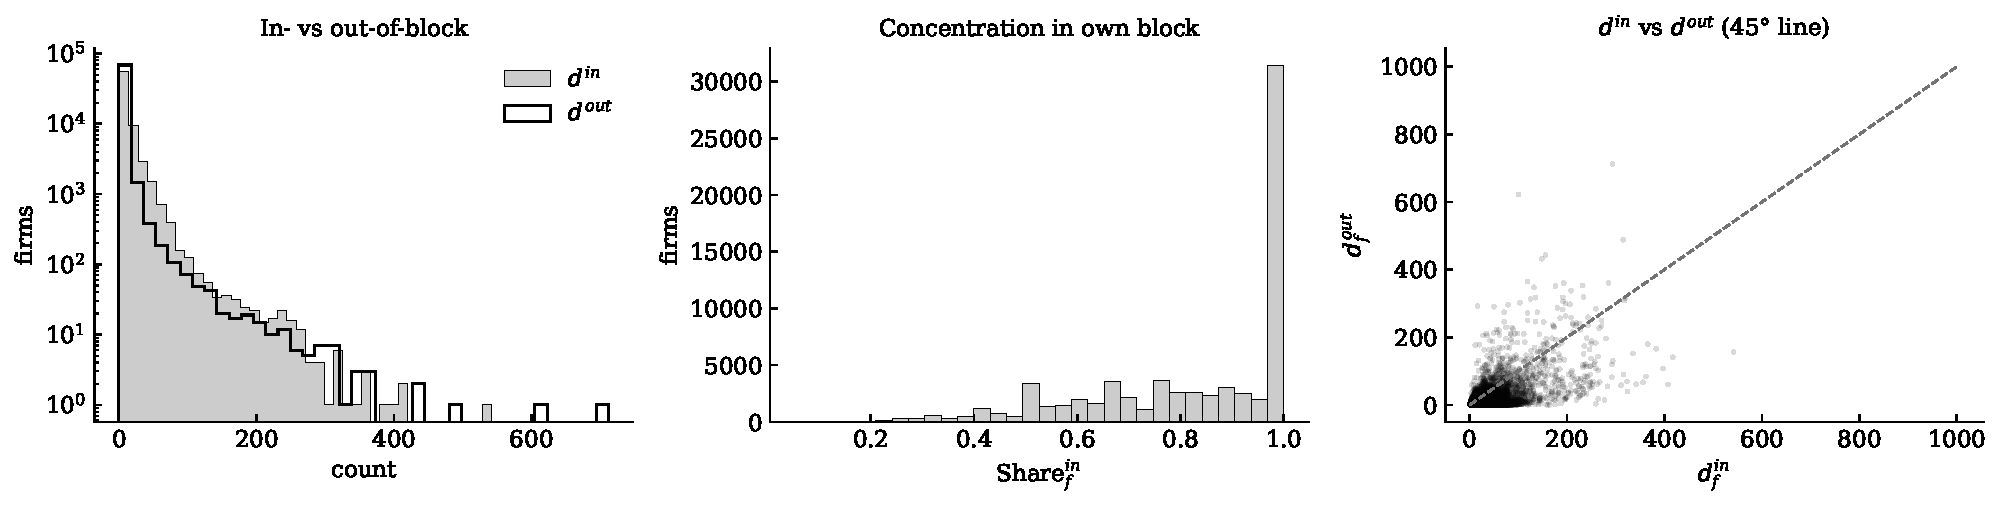
\includegraphics[width=0.99\textwidth]{ds_g2_diversification.pdf}
\caption{$\gamma=2$ diversification triptych, to compare with Fig.~\ref{fig:div} ($\gamma=1$). \textbf{Left:}
in- vs out-of-block counts (log $y$), $\dout$ shifted up. \textbf{Centre:} $\mathrm{Share}^{\mathrm{in}}$ ---
a smaller mass at $1$ than at $\gamma=1$ ($43.2\%$ vs $54.5\%$). \textbf{Right:} $\din$ vs $\dout$ with the
$45^\circ$ line --- more firms now sit above the axis, but the cloud stays below the diagonal.}
\label{fig:g2div}
\end{figure}

\begin{figure}[H]\centering
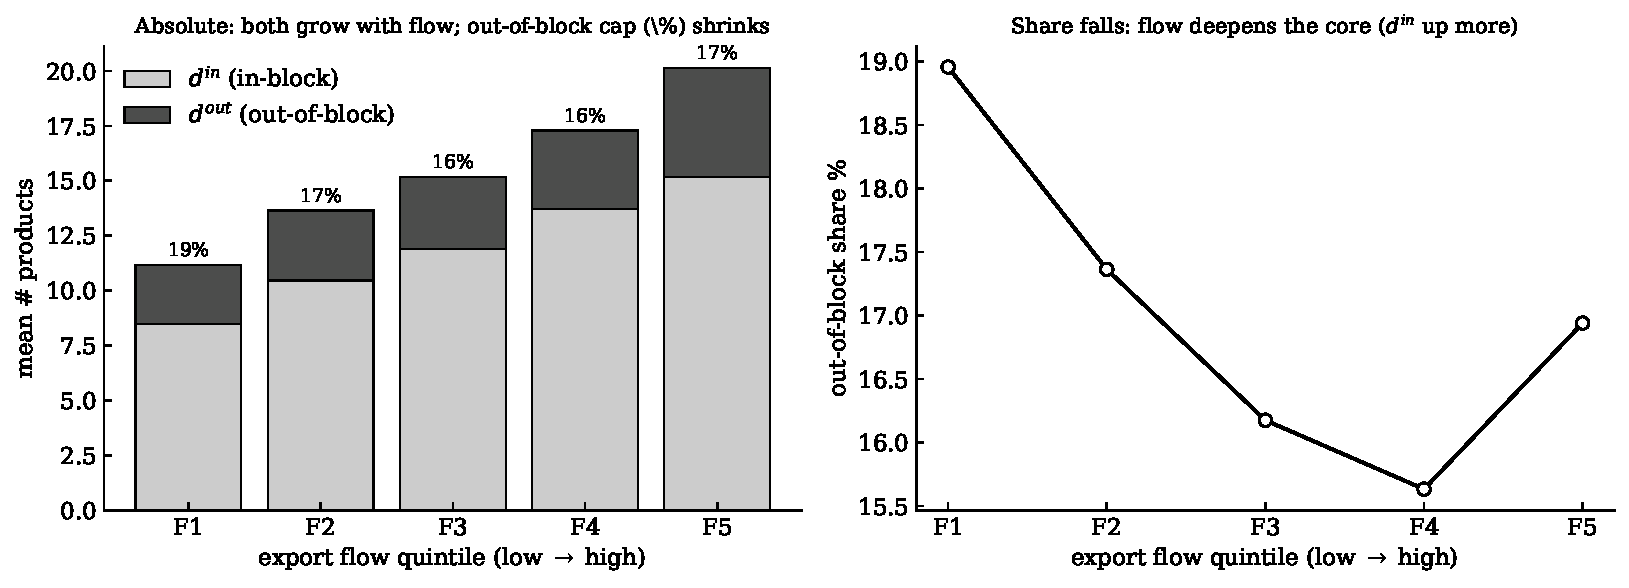
\includegraphics[width=0.97\textwidth]{ds_g2_flow_mechanism.pdf}
\caption{$\gamma=2$ flow mechanism (destination reach held fixed), to be read against the $\gamma=1$ version
(Fig.~\ref{fig:mech}). \textbf{Right:} the out-of-block share falls with flow only up to F4 and then
\emph{rebounds} at the top flow quintile F5 --- the one place the ``volume deepens the core'' reading breaks
under a finer partition.}
\label{fig:g2mech}
\end{figure}

%=================================================================
\section{Keep attention for the dynamic landscape}

These are the emphasis points from the static analysis worth keeping in mind for the dynamic, tariff-driven
part:

\begin{itemize}
  \item \textbf{Freeze the partition.} Estimate the blocks once (pre-period or pooled) and hold them fixed;
        otherwise $\din/\dout$ become endogenous to the shock and the treatment is absorbed into the partition.
        Let only the portfolio $E_{fp}(t)$ vary: $\din(t)=\sum_p E_{fp}(t)\,\delta_{fp}$.
  \item \textbf{Measure within-firm variation first.} A fixed-effects panel identifies off within-firm
        movement; the year-to-year variance of $\din,\dout,$ share is not yet known and decides power.
  \item \textbf{Pick outcomes by their distribution.} $\din$ is cleanest; $\dout$ is zero-inflated
        ($54.5\%$ zeros) $\to$ PPML; the share is floor/ceiling-bound, so the falsifier ($\dout$ up) is better
        powered than retrenchment (share up, $\dout$ down).
  \item \textbf{Heterogeneity by destination reach.} Out-of-block exploration lives in wide-reach (not
        high-volume) firms (\S\ref{sec:dest}) and in particular blocks (\S\ref{sec:blocks}); let effects vary by
        reach and track the product and geographic margins jointly.
  \item \textbf{Control for intermediaries with coherence.} Low coherence flags wholesalers with spurious
        $\dout$; condition on $C_f$ or trim the low-coherence tail.
  \item \textbf{Carry the sample caveats.} Balanced core only ($19\%$ of firms, $62\%$ of value); block
        \emph{count} is resolution/algorithm-dependent, so fix the partition choice (BRIM, $\gamma=1$).
\end{itemize}

%=================================================================
%=================================================================
\section*{Appendix: community-detection algorithms and the resolution $\gamma$}
\label{app:algos}
\small

All three algorithms partition the \emph{same} bipartite firm--product graph, but they optimise different
objectives, and the difference is entirely in the \emph{null model} --- the random baseline against which
observed within-block links are scored.

\paragraph{Modularity and the null.} Modularity rewards a partition for the links that fall inside blocks
\emph{beyond} what a degree-preserving random graph would put there. For a one-mode graph (Newman, 2006),
$Q=\frac{1}{2m}\sum_{ij}\big(A_{ij}-\gamma\,\tfrac{k_ik_j}{2m}\big)\delta(c_i,c_j)$, where $k_ik_j/2m$ is the
configuration-model expectation and $\gamma$ the resolution.

\paragraph{Louvain (Blondel et al., 2008).} A fast greedy optimiser of the one-mode $Q$. Run on a bipartite
graph it still uses the \emph{one-mode} null, which expects firm--firm and product--product links that cannot
exist; the mis-specified baseline inflates apparent within-block density and Louvain tends to
\emph{over-segment} (here: 13 blocks).

\paragraph{Leiden (Traag et al., 2019).} An improved optimiser that repairs Louvain's badly-connected-community
defect and guarantees well-connected blocks. We run it on the same one-mode RB-modularity: a better optimiser,
but the same null mis-specified for a two-mode graph (here: 9 blocks).

\paragraph{BRIM (Barber, 2007).} Uses the \emph{correct bipartite null}. The expected link between firm $f$ and
product $p$ is $k_f d_p/m$ --- it preserves the firm and product degree sequences separately and places expected
links only across the two node types, never within one. The bipartite modularity is
$\QB=\frac{1}{m}\sum_{fp}\big(B_{fp}-\gamma\,\tfrac{k_f d_p}{m}\big)\delta(g_f,g_p)$, and blocks are co-clusters
containing both firms and products. This is De Stefano's choice and ours (here: 5 blocks, $\QB=0.505$). We
implement it through \texttt{leidenalg}'s CPM-bipartite recipe, scaled so that $\gamma=1$ reproduces standard
Barber modularity.

\paragraph{The resolution $\gamma$.} $\gamma$ multiplies the null term --- the ``charge'' for grouping two nodes
--- so $\gamma=1$ is standard modularity, $\gamma>1$ gives more and smaller blocks, $\gamma<1$ fewer and larger.
In the CPM form $\gamma$ is a density threshold (keep a community only if its internal density exceeds
$\gamma$), which is why CPM avoids the modularity resolution limit. Leiden is only the optimiser; $\gamma$
belongs to the objective. We keep $\gamma=1$ as the baseline and report $\gamma=2$ in \S\ref{sec:gamma}.

%=================================================================
\section*{References}
\footnotesize
\begin{itemize}[leftmargin=1.4em,labelsep=0.4em]\raggedright
  \item Albora, G., Rossi Mori, L., Zaccaria, A. (2023). Sapling Similarity: a performing and interpretable memory-based tool for recommendation. arXiv:2210.07039.
  \item Balassa, B. (1965). Trade liberalisation and ``revealed'' comparative advantage. \emph{The Manchester School} 33(2): 99--123. doi:10.1111/j.1467-9957.1965.tb00050.x
  \item Barber, M. J. (2007). Modularity and community detection in bipartite networks. \emph{Physical Review E} 76(6): 066102. doi:10.1103/PhysRevE.76.066102
  \item Blondel, V. D., Guillaume, J.-L., Lambiotte, R., Lefebvre, E. (2008). Fast unfolding of communities in large networks. \emph{Journal of Statistical Mechanics} P10008. doi:10.1088/1742-5468/2008/10/P10008
  \item De Stefano, V., Mula, M., Mariani, M. S., Zaccaria, A. (2025). From macro to micro: economic complexity indicators for firm growth. arXiv:2507.21754.
  \item Hausmann, R., Hwang, J., Rodrik, D. (2007). What you export matters. \emph{Journal of Economic Growth} 12(1): 1--25. doi:10.1007/s10887-006-9009-4
  \item March, J. G. (1991). Exploration and exploitation in organizational learning. \emph{Organization Science} 2(1): 71--87. doi:10.1287/orsc.2.1.71
  \item Newman, M. E. J. (2006). Modularity and community structure in networks. \emph{Proceedings of the National Academy of Sciences} 103(23): 8577--8582. doi:10.1073/pnas.0601602103
  \item Tacchella, A., Cristelli, M., Caldarelli, G., Gabrielli, A., Pietronero, L. (2012). A new metrics for countries' fitness and products' complexity. \emph{Scientific Reports} 2: 723. doi:10.1038/srep00723
  \item Traag, V. A., Waltman, L., van Eck, N. J. (2019). From Louvain to Leiden: guaranteeing well-connected communities. \emph{Scientific Reports} 9: 5233. doi:10.1038/s41598-019-41695-z
\end{itemize}

\end{document}
